\chapter{Modular networks throughout development}

\section{Motivation}

Childhood represents the ideal time window in which to study the relationship of brain network architecture on reading because of the rapid changes and growth. Over the first three studies, we found that whole-brain modularity was predictive of reading skill and conserved during reading comprehension but that there was an increase in integration among RSNs during reading. RSNs related to attention and internal thinking, including the dorsal attention, ventral attention and default mode networks were especially impacted. Reduced modularity was not unique to the reading process, however, and we found a high degree of similarity, on average, when comparing several different network structures within each individual -- roughly one third of connections were conserved. 

Despite the benefits of studying children, it is important to couch these findings in a developmental context: for example, does higher modularity and network consistency represent a more mature architecture, or is it tied to individual variability in organization? Although we are just beginning to understand how maturation changes the network architecture of the brain, there have been some consistent findings in the past several years. One of the earliest findings was that in children, short-range connections are strongest, whereas in adults, long-term connections increase in strength \citep{Power2010, Chan2014}. This is accompanied by decreases in functional network modularity and the coherence (fractional anisotropy) of white matter tracts, and in later life, decreases in the participation coefficients of hub areas \citep{Betzel2014}. It should be noted, however, that many of these lifespan studies have investigated the time period between early adulthood and senescence, with fewer studies having been done in childhood and adolescence \citep{Cao2016}.

One purported benefit of a modular brain architecture is ``evolvability'': the capacity for a system to easily adapt to environmental circumstances because new modules can be added without drastically altering the other modules \citep{Kashtan2005}. Each one can work in parallel, sharing information when necessary, but without being too dependent on the success or failure of another system. This makes modularity not only efficient and robust to damage, but also capable of accommodating change over the lifespan. Cognition, too, has traditionally been considered to a large degree modular, with the pseudo-science of phrenology being the most extreme example, but more recent efforts coming from a deeper understanding of visual and sensory systems \citep{Barrett2006}. However, some higher-order cognitive functions such as working memory, attention and planning have not been localized to a discrete cortical area and are more likely to depend on a global workspace \citep{Dehaene1998}.

The degree of reorganization is likely to depend on the individual's ability to respond to a given task. Although it is still an area of investigation, one group investigated how modularity changed over the course of learning a novel task. Bassett and colleagues scanned participants at four timepoints while they were learning a new finger-tapping task: before training, early in training, midway through training and at the end of training \citep{Bassett2015}. The authors empirically defined a visual and motor module, and investigated changes to it throughout training. They found two important trends: first, the two modules became increasingly segregated throughout training and practice; and second, the involvement of non-module nodes such as those in subcortical systems was reduced over time. A separate study found that that modules are more likely to re-organize at early stages in the training process \citep{Bassett2010}. Taken together, the findings suggest a model in which the early stages of training require a high degree of cross-module communication, whereas later stages rely on more automated, modular processes (i.e. efficient and segregated processing). 

The cognitive processes in reading are also thought of in a modular sense: visual, auditory, semantic and motor processes can each be taught or assessed separately. Phonics instruction focuses on letter-sound mapping, a process which engages both auditory and visual systems. Neuroimaging evidence from the past two decades suggest that this binding process localizes to specific areas, including the left temporo-parietal junction and visual word form area \citep{Price2012}. These areas have received a lot of focus because they serve as bottlenecks for reading efficiency which, if they have not been tuned properly, prevent fluent reading. However, there have also been efforts to characterize poor reading as a lower-level deficit in terms of more fundamental processes, including visuo-spatial attention \citep{Vidyasagar2010}, cerebellar function \citep{Pernet2009, Eckert2003},  subcortical sensory processing \citep{Stein1997, Fan2014}, or some combination of these \citep{Pernet2009}. We suggest that global modularity in the context of reading skill is best interpreted as high efficiency in these more basic processes. 

In this chapter, we seek to further develop our model of the relationship between network architecture and reading by investigating changes throughout development. We use task-based methods previously described (but with new stimuli) to attempt a replication of previous findings in a new cohort of subjects.  We then explore the differences in network organization during reading comprehension. Finally, we use the reference-free methods of similarity described in Chapter 4 to investigate within- and between-subject flexibility of network architecture. 
We note that, although the data analyzed here parallel those described in Studies 1, 2 and 3, this also introduces some challenges. Most important of these is that developmental effects are confounded by the task difficulty and differences in motion. Even with these limitations, however, the results will provide important context for our previous findings and help to flesh out a model of the advantages conferred to specific cognitive skills by the modular brain.


\section{Methods}

\subsection{Participants}

Participants in this study were drawn from several studies and age groups to represent a cross-section of the population at different points in development. They fell into three categories: a group of children (ages 8 to 10) were selected from the third wave of the longitudinal study described in Study 1;  a group of adolescents (ages 10 to 14) from a large, cross-sectional study on the cognitive components of reading; and a group of adults (ages 18 to 40), largely from a population of university research assistants and graduate students. In this final group, behavioral data was sparsely collected, so no analyses of reading-related skill are possible. Demographics for these subjects are described in Table \ref{table:ch5-participants}.

\begin{table}[t]
	\renewcommand{\tabcolsep}{0.09cm}
	\centering
	\begin{tabular}{lll}
\toprule
Measure &               Young Group &               Mature Group \\
\midrule
Subjects                        &              38 &              38 \\
Total scan runs                 &             118 &             136 \\
Mean age                        &     9.38 (0.31) &    19.16 (7.99) \\
Sex                             &      18 M, 20 F &      21 M, 17 F \\
Individuals with Testing		& 			  38 &				18	\\
WASI Full-Scale IQ, Vocabulary  &   55.37 (11.95) &    55.89 (7.52) \\
Test of Word Reading Efficiency &  109.95 (15.23) &  101.33 (15.50) \\
\bottomrule
\end{tabular}
	\caption[Participant demographics for Study 4]{Participant demographics for Study 4. Participants were drawn from three samples: children from the third wave of the longitudinal study described in Studies 1 to 3; adolescents in a cross-sectional study of reading comprehension skill; and adult volunteers. Scan sessions followed the same task design as in Study 3 but stimuli were novel.}
	\label{table:ch5-participants}
\end{table}

\subsection{Functional MRI acquisition and processing}

The task design for this study is described in detail in Chapters 3 and 4. Briefly, subjects were presented up to four separate runs of a language comprehension task. The task included two passage blocks (``reading'' or ``listening''), two sensory baseline blocks (``symboles'' or ``tones'') and a trailing resting-state block (``rest''). The four scan runs were crossed on two conditions: the modality of presentation (auditory or visual) and the genre of the passage (narrative or expository). One difference, however, was that the contents of the passages presented to these participants differed from those previously described. While still balanced to a third-grade reading level using Coh-Metrix, the passages were novel. 

Motion is a major confound in age-related connectivity analyses since, on average, children move much more during a given scan session than their older counterparts. To combat this, we applied a stricter motion criteria for inclusion than previously: subjects needed to have no more than 10 percent outlier volumes across the entire scan. A total of 72 unique subjects and 256 scan sessions met this criteria. 

Functional MRI acquisition and preprocessing procedures were equivalent to those described for Studies 2 and 3. See the \textit{Methods} section of Chapter 3 for a detailed description of these processes and their parameters.

\subsection{Network analyses}

Analyses were broken into three parts. First, we sought to understand what effects development had on the modularity of the brain at rest and during reading. We assessed these changes by analyzing the task-evoked networks for each of our participants, and using the group (children, adolescents, adults) and task conditions (rest, symbols, reading) as the factors in a two-way ANOVA predicting network modularity. We then analyzed changes to connectivity strength at the connection- and RSN-level to summarize changes to reading-evoked activity across development. For these analyses, we created connectivity networks (thresholded to retain the top 5 percent of connections) for each subject's ``reading'' connectome, then we performed an independent two-sample $t$-test between younger readers (Group 1) and older readers (Groups 2 and 3) on each connection. For each RSN-RSN pair, we summed all connections that were significant at an uncorrected $p < 0.05$ to create a measure of net connectivity change between the two RSNs.

We also sought to replicate previous results showing a positive relationship between global modularity and reading. In particular, we sought to determine whether this relationship changed over time (for example, flattening out in older readers). For this study, we used the average modularity during the resting condition of the task. (Data could be drawn from either 2 or 4 sessions, or approximately 8 - 16 minutes of resting-state signal). The adult group had an inconsistent amount of data available, so this regression analysis was only able to be performed across Groups 1 and 2.

Finally, we built upon Study 3 by investigating how network similarity changes throughout development. We had two questions: first, whether between-subject similarity increases over time, and second, whether the mature network is more ``flexible'' and reorganizes itself to a greater degree during different tasks than younger individuals. To accomplish these two objectives, we calculated the intersection of the union for each subject's reading-evoked network with each of their peers (Group 1 to Group 1, etc.). (We also did this for their resting-state network.) We then averaged this IOU metric and performed a $t$-test between the younger and older participants. To study within-subject variability, we followed the methods described in Chapter 4: for each of the six conditions that each subject (reading, listening, symbols, tones and rest in each modality), we calculated the pairwise similarity matrix, then averaged it. Higher mean values indicate a higher level of similarity between each evoked state. We then performed a $t$-test between younger and older subjects.


\section{Results}

% Scan inclusion
In total, 76 subjects (254 scan runs) were analyzed. Despite our stricter criteria, motion does represent a potentially confounding variable for between-group comparisons, as there was significantly less motion in Group 3 (adults). As discussed in Study 1, however, we have attempted to address these differences through preprocessing techniques.

% Modularity across time and modality age
We first tested the effects of task condition and age on estimates of modularity on the reading comprehension task. We set up a two-way ANOVA with the three groups (young readers, adolescents, adults) as one factor and the three experimental conditions (rest, symbols, reading) as the other factor. Figure \ref{fig:ch5-modularity-by-condition-3groups} displays the distribution of these data. 

\begin{figure}[t]
	\centering
	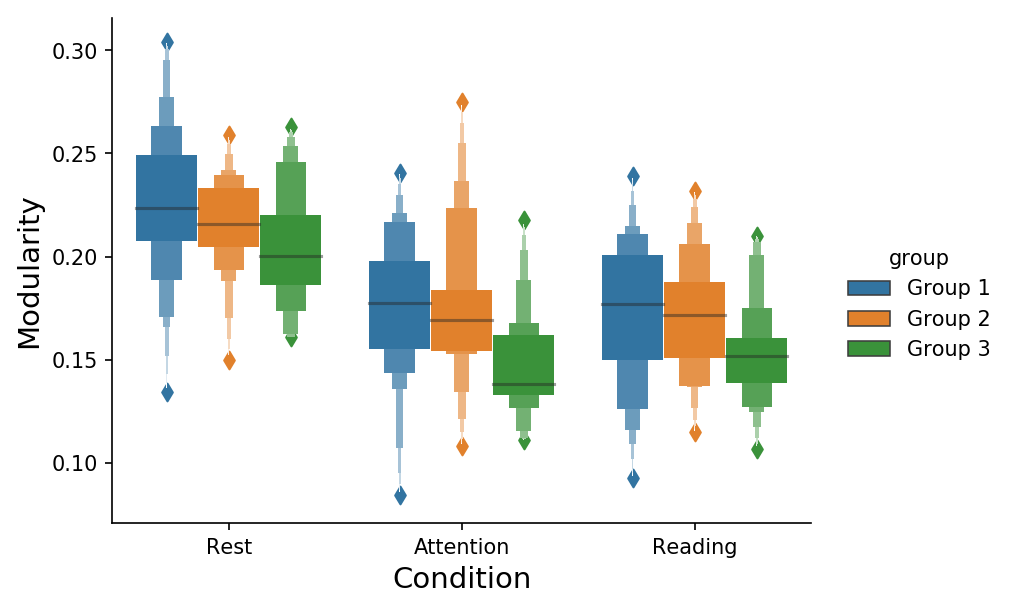
\includegraphics[width=5.5in]{ch5-modularity-by-condition-3groups}
    \caption[Adults have lower modularity but undergo the same task effects as younger readers]{Adults have lower modularity but undergo the same task effects as younger readers. For the group factor, adults ('Group 3') had a lower modularity than the younger participants, but Groups 1 and 2 were not significant different. For experimental conditions, resting state had a higher modularity than both task conditions, which did not differ significantly.}
	\label{fig:ch5-modularity-by-condition-3groups}
\end{figure}

We found significant main effects for both group ($F = 11.376$, $p < 0.001$) and condition ($F = 60.4$, $p < 0.001$), but not their interaction ($F=0.470$, $p = 0.758$). We then conducted post-hoc $t$-tests on the comparisons within each factor. With regard to group effects, adults had a lower modularity than the younger participants, but Groups 1 and 2 were not significant different. For experimental conditions, resting state had a higher global modularity than both task conditions, which did not differ significantly. See Table \ref{table:ch5-modularity-age-condition} for complete results. 

\begin{table}[t]
	\renewcommand{\tabcolsep}{0.09cm}
	\centering
	\begin{tabular}{lrrrr}
\toprule
Variable &    Sum. of Squares &     Deg. Freedom &          $F$ / $t$ &        $p$-value \\
\midrule
\textsc{Two-Way ANOVA} 	& 	& & & \\
Group                   &  0.023 &    2 &  11.374 &  $< 0.001$ \\
Condition               &  0.126 &    2 &  60.402 &  $< 0.001$ \\
Group:Conditions 		&  0.001 &    4 &   0.469 &  $0.758$ \\
Residual                &  0.229 &  219 &        --- &           --- \\
& & & & \\
\textsc{Post-Hoc $t$-tests} & & & & \\
\textit{Conditions} & & & & \\
Rest > Attention  	&  ---  &    ---- &  13.341 &  $< 0.001$ \\
Rest > Reading  	&  ---  &    ---- &  14.279 &  $< 0.001$ \\
Attention > Reading &  ---  &    ---- &  0.437 &  $0.663$ \\
\textit{Groups} & & & & \\
Group 1 > Group 2  &  ---  &    ---- &  0.604 &  $0.546$ \\
Group 1 > Group 3  &  ---  &    ---- &  3.733 &  $< 0.001$ \\
Group 2 > Group 3  &  ---  &    ---- &  2.869 &  $0.005$ \\
\bottomrule
\end{tabular}
	\caption[Statistical results for the effects of condition and group on modularity]{Two-way ANOVA table for the main effects of condition and group on modularity. Below are results for post-hoc $t$-tests conducted within each factor.}
	\label{table:ch5-modularity-age-condition}
\end{table}

% Similarity across all conditions over time
Next, we turned to individual differences in RSN connectivity to understand drivers of decreased modularity. We first examined changes at the connection-level by comparing the strength (i.e. correlation) between the younger and older groups. We noted two spatial trends: there is greater connectivity strength in posterior areas in the younger group, whereas the older group shows greater connectivity between anterior and bilateral areas. See Figure \ref{fig:ch5-group-difference-connections} for a diagram of these connections.

\begin{figure}[t]
	\centering
	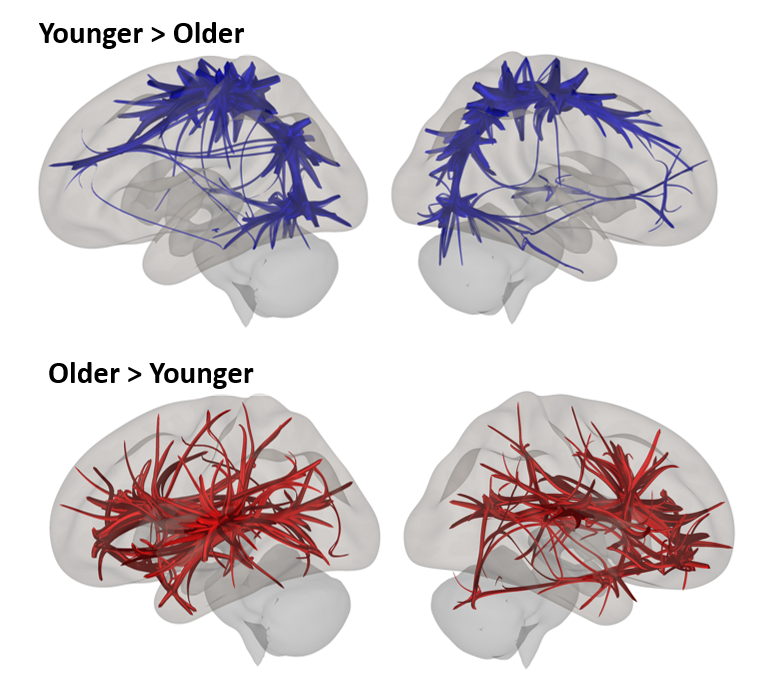
\includegraphics[height=4.5in]{ch5-group-difference-connections}
    \caption[Connection-level changes in the reading network]{Connection-level changes to the reading network. Connections that showed significant differences between older and younger readers. Dorsal and posterior connections had higher connectivity strength in younger readers than anterior and bilateral connections. Connections shown here are significant at $p < 0.05$, FDR-corrected.}
	\label{fig:ch5-group-difference-connections}
\end{figure}

To summarize this at the RSN level, we grouped each significant connection by its originating and target RSN, then summed up the number of connections changed. The net results of this aggregated connectivity map are shown in Figure \ref{fig:ch5-group-difference-rsn-connectivity}. This map reveals a few important trends: when children read, there is high connectivity within and between the dorsal attention, visual, somatomotor and executive networks. In older readers, the concentration of connections shifts towards higher-order areas such as the default mode and salience network, as well as the auditory and ventral attention areas.  In the context of our previous findings, it would seem that mature readers have a reduced modularity due to decreased within-network connectivity of visual, somatomotor and dorsal attention networks.

\begin{figure}[t!]
	\centering
	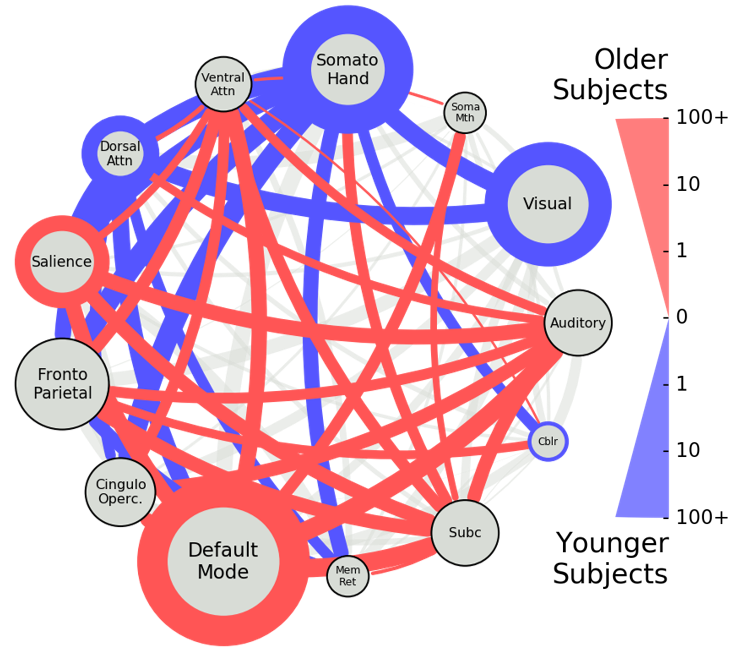
\includegraphics[height=4.5in]{ch5-group-difference-rsn-connectivity}
    \caption[Developmental shifts in RSN interactivity]{Developmental shifts in connectivity strength. When children read, there is greater connectivity within and between the dorsal attention, visual, somatomotor and executive networks. In older readers, the concentration of connectivity shifts towards ventral attention, salience and the default mode networks.}
	\label{fig:ch5-group-difference-rsn-connectivity}
\end{figure}

% Modularity to reading
We then attempted to replicate our findings that higher global modularity at rest was associated with higher reading skill. We were unable to test the relationship in the oldest readers (ages 15 and older), but did have access to TOWRE scores from participants in Group 2. When all subjects were included in the analysis ($n$ = 56), there was a positive correlation that trended toward significance but did not quite reach it ($r = 0.256$, $p = 0.057$). When analyzed separately, we found that the correlation was higher in younger readers ($r=0.280$, $p=0.089$) than older readers ($r=0.198$, $p=0.432$). 

We noticed that some of the poorest readers had more variability in their modularity values. We re-ran the correlations excluding the 4 readers with standard scores of 85 or less (one standard deviation below average, or the bottom 16 percent). This adjustment made the correlation across the entire group ($r = 0.404$, $p = 0.003$) and the younger group ($r = 0.459$, $p = 0.006$). Although the correlation increased for the adolescent group, it did not reach significance either ($r = 0.292$, $p = 0.273$).

\begin{figure}[t]
	\centering
	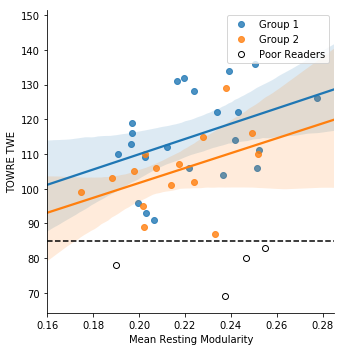
\includegraphics[height=3in]{ch5-modularity-reading-corr-2groups}
    \caption[Modularity is related to reading skill in younger readers]{Modularity is related to reading skill in younger readers. Although including all developing readers resulted in a significant correlation, and both Groups 1 and 2 had positive correlations with reading skill, the relationships only reached signifiance in Group 1 when analyzed separately. It is also possible that this relationship is different in very poor readers (e.g. bottom 16 percent, as shown here).}
	\label{fig:ch5-modularity-reading-corr-2groups}
\end{figure}

% Similarity betwen listening and reading over time
Finally, we investigated how subject ``flexibility'' differed across age groups. We first compared the degree of subject similarity between ``developing readers'' (Group 1) and ``mature readers'' (Groups 2 and 3) during reading and rest. Consistent with our findings of decreased modularity, we found that older participants had, on average, lower similarity to their peers than children did. This was true both during language comprehension ($t = 13.829$, $p < 0.001$) and at rest ($t = 9.087$, $p < 0.001$). Figure \ref{fig:ch5-pairwise-iou-reading} provides an example of this effect for the reading-evoked network.

\begin{figure}[t]
	\centering
	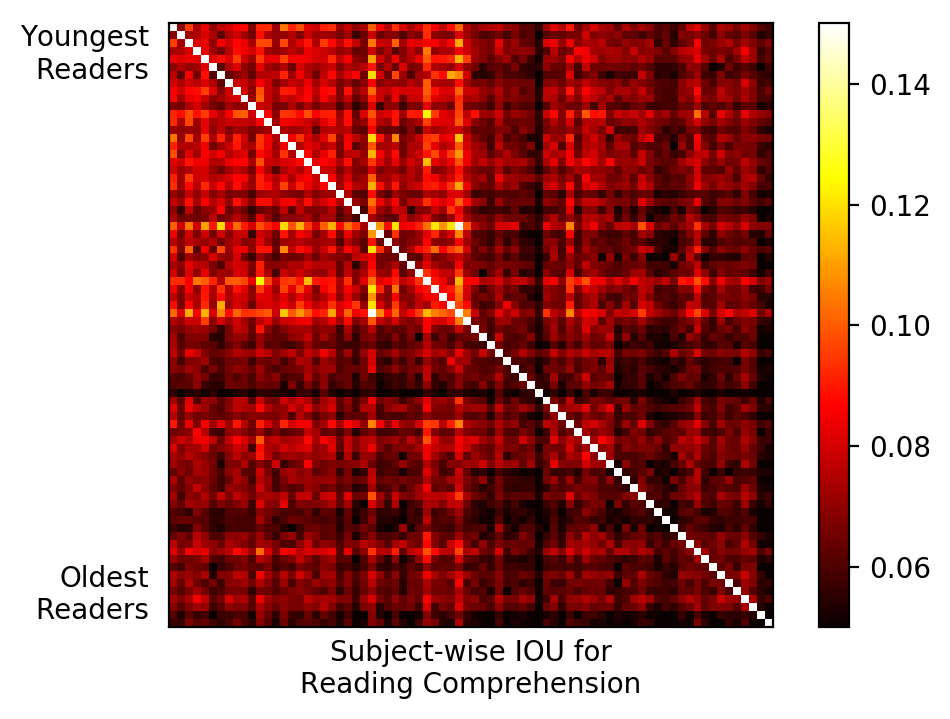
\includegraphics[height=3in]{ch5-pairwise-iou-reading}
    \caption[Older subjects show less similarity between in reading-evoked networks]{Older subjects show less similarity between in reading-evoked networks. Network similarity decreased in the older group, even as within-subject similarity stayed the same. This suggests that, while older subjects largely retain the modular architecture from early in life, they also develop a more individualized connectome.}
	\label{fig:ch5-pairwise-iou-reading}
\end{figure}

Despite the findings of decreased modularity, we found no evidence that the the within-subject IOU across conditions changed ($t = 0.239$, $p = 0.811$). This was also true of the comparison of the listening-evoked to reading-evoked networks, which were previously found to be correlated with reading skill. This level of similarity was consistent across all age groups and had a mean of 0.345 (standard deviation of 0.047), replicating the results from Chapter 4 (mean similarity of 0.364).

\section{Discussion}

% Summary of findings
In this study, we sought to better understand how the maturation of the human brain affects functional network architecture and its reorganization during tasks. We build on our previous work showing that the modular organization of the brain decreases slightly throughout the lifespan but is similarly disrupted during tasks, no matter the age or expertise of the individual. We identified developmental shifts in network connectivity which show that an emphasis on sensorimotor and dorsal attention systems gives way to connectivity between default mode, auditory, ventral attention and salience systems. While the within-individual variation of task-evoked and resting-state architecture remained consistently high in mature participants, adult networks showed a greater amount of variability than in children. The results bolster the hypothesis that modularity is an adaptive trait which allows for growth and the support of cognitive functioning throughout the lifespan.

% Similarity across all conditions over time
Although the global differences between reading and rest remained the same throughout development, there were major changes in the manner with which they reorganized. The adult connectivity network had fewer connections in visual, dorsal attention and somatomotor areas. This is consistent with previous findings of decreased modularity of visual, dorsal attention and control regions in later life \citep{Betzel2014}.  One interpretation is that children were more sensory-laden: they used their top-down attention systems to focus more on the mechanics of reading. Adults, on the other hand, had a more anterior and bilateral network. The significant increases of connectivity within the default mode network certainly support the hypothesis that adults had richer internal mental activity during the stories \citep{Spreng2013}. That is, they may have been better able to focus on the content and integrate it with more of their personal experiences and background knowledge. We also note in particular the differences in connectivity between the dorsal attention and ventral attention networks. In Study 2, we saw that the ventral attention network is a critical reading-related RSN, and in adults we observe that it is connecting out to a number of higher-order processing areas. This supports the idea that adults have automated much of the lower-level visual processing of reading such that the ventral attention network can feed it up to other systems \citep{Twomey2011}.

% Modularity throughout the lifespan
Some models of network development suggest that children have intact network architectures from early on in life and RSNs with long-range connections, such as those in the fronto-parietal and cingulo-opercular, strengthen later in life \citep{Uddin2010, Cao2016}. Our findings are compatible with such a model but extend it in two ways. First, the finding of greater modularity in children also means that younger subjects were more similar to the reference partition from Power and colleagues \citep{Power2011}. This reference partition is the result of finding a consensus parcellation across nearly 100 subjects, suggesting that children more closely resemble the ``average'' brain network than adults. Second, adults shared fewer similarities to other adults than children did to other children, but showed strong consistency within themselves. In effect, their within-person modularity was just as high as it was in children.

% The developmental model
It thus appears that humans start life with an archetypal architecture  and ``tweak'' it as they learn and grow. In fact, this is the evolutionary advantage of modularity: a system can easily adapt to its environmental circumstances because new modules can be added without drastically altering the other modules \citep{Kashtan2005}. Individuals can add new skills, such as recognizing a new alphabet, or rewire portions of cortex to perform new functions, as in stroke recovery, without having to re-build the system from the ground up. Indeed, this is what happens in the case of literacy: locations predisposed to be useful for connecting areas (e.g. fusiform gyrus) are recycled for more specific uses \citep{Saygin2016}. It's likely that this process occurs consistently throughout development and even in less ``revolutionary'' skills than reading, as John Steinbeck puts it. This process of continual editing and adding results in a more individualized architecture in adulthood, even though the template remains the same. 

% Limitations
Although this study boasts several major features, including the replication of previous results, multiple cross-sectional age groups and a large number of analyzed scans (254 scans totalling nearly 30 hours of scan time), there are a few limitations. First of all, the passages were balanced to a third grade reading level, meaning that the younger groups may have found them challenging while the older groups found them very easy. While this is likely, we do not believe this unduly influences the results. The passages were presented at a pace that was slow enough for the young readers to follow along without difficulty, and they were also presented phrase-by-phrase so that older readers would still have to engage with the text for the same amount of time and retain a mental model over the same period. More pernicious may be the differences in scan motion between the two groups. However, we have included a narrower portion of the young population and also performed several layers of preprocessing to account for these effects.   

% Modularity ties into reading
We were able to replicate our findings that higher global modularity is correlated with better reading skill, with two new findings. First, the strength of the connection seems to decrease as children get older and reach adolescence. This might reflect the individuation of their architecture, as discussed above, or it could be that the effects of experience begin to trump an intrinsic biological disposition. The relationship was greatly strengthened in the younger group when we excluded very poor readers from analysis. One possibility is that individuals who struggle may have focal differences, such as in phonological processing, that are not reflected in the global architecture. We interpret a highly modular brain as one with many very efficiently organized sub-systems. One potential intersection this model has with reading is that this may reflect the importance of the ``building blocks'' of reading. Rather than reading (and reading difficulty) being defined by the activity of a few important areas (for example, the occipito-temporal cortex, temporo-parietal junction, inferior frontal gyrus), the integrative process relies on finely tuned RSNs. These may correspond with cognitive skills such as visual attention and phonological awareness. Any inefficiencies in these basic skills will cascade into problems integrating into the larger network.